\documentclass[12pt, leqno]{article} %% use to set typesize
\usepackage{fancyhdr}
\usepackage[sort&compress]{natbib}
\usepackage[letterpaper=true,colorlinks=true,linkcolor=black]{hyperref}

\usepackage{amsfonts}
\usepackage{amsmath}
\usepackage{amssymb}
\usepackage{color}
\usepackage{tikz}
\usepackage{pgfplots}
\usepackage{listings}
%\usepackage{courier}
%\usepackage[utf8]{inputenc}
%\usepackage[russian]{babel}

\lstset{
  numbers=left,
  basicstyle=\ttfamily\footnotesize,
  numberstyle=\tiny\color{gray},
  stepnumber=1,
  numbersep=10pt,
}

\newcommand{\iu}{\ensuremath{\mathrm{i}}}
\newcommand{\bbR}{\mathbb{R}}
\newcommand{\bbC}{\mathbb{C}}
\newcommand{\calV}{\mathcal{V}}
\newcommand{\calW}{\mathcal{W}}
\newcommand{\macheps}{\epsilon_{\mathrm{mach}}}
\newcommand{\matlab}{\textsc{Matlab}}

\newcommand{\ddiag}{\operatorname{diag}}
\newcommand{\fl}{\operatorname{fl}}
\newcommand{\nnz}{\operatorname{nnz}}
\newcommand{\tr}{\operatorname{tr}}
\renewcommand{\vec}{\operatorname{vec}}

\newcommand{\vertiii}[1]{{\left\vert\kern-0.25ex\left\vert\kern-0.25ex\left\vert #1
    \right\vert\kern-0.25ex\right\vert\kern-0.25ex\right\vert}}
\newcommand{\ip}[2]{\langle #1, #2 \rangle}
\newcommand{\ipx}[2]{\left\langle #1, #2 \right\rangle}
\newcommand{\order}[1]{O( #1 )}

\newcommand{\kron}{\otimes}


\newcommand{\hdr}[1]{
  \pagestyle{fancy}
  \lhead{Bindel, Summer 2018}
  \rhead{Numerics for Data Science}
  \fancyfoot{}
  \begin{center}
    {\large{\bf #1}}
  \end{center}
  \lstset{language=matlab,columns=flexible}  
}


\begin{document}
\hdr{2018-06-26}

% A test case: polynomial approximation
% - Stone-Weierstrass to Jackson inequality
% - Intermediate functions and polynomial interpolation

% Piecewise linear functions and DNNs
% Piecewise cubic functions and splines

\section{Approximation and models}

Suppose $f : \bbR^n \rightarrow \bbR$.  The basic problem in function
approximation is to find a function $\hat{f}$ from some family
so that $f$ and $\hat{f}$ are ``close.''  For example, we might seek
to approximate $f$ by a linear function, a polynomial, a piecewise
polynomial, a deep neural network, of a kernel-based approximation.
To measure closeness, we usually use some norm on functions;
like norms on finite-dimensional vector spaces, norms on spaces
of function give us a way of measuring the a function's size.
Some common choices are the max norm (or $\infty$ norm)
\[
  \|f-\hat{f}\|_{L^\infty(\Omega)} = \max_{x \in \Omega} |f(x)-\hat{f}(x)|,
\]
the Euclidean norm with respect to some measure $\mu$
\[
  \|f-\hat{f}\|_{L^2(\mu)}^2 = \int |f(x)-\hat{f}(x)|^2 \mu(x) \, dx,
\]
or the one norm with respect to some measure $\mu$
\[
  \|f-\hat{f}\|_{L^1(\mu)} = \int |f(x)-\hat{f}(x)| \mu(x) \, dx.
\]
When the domain or the measure is obvious, we will sometimes write
these norms more tersely as $\|\cdot\|_\infty$, $\|\cdot\|_2$, and
$\|\cdot\|_1$.  Of course, other norms are possible as well, and we
will see some of them in our discussions.
Different norms make sense for different scenarios --- and we have to
make sure to restrict our attention to functions for which the norms
are well-defined!  And beyond an error that is small in some norm, we may also
want other properties for $\hat{f}$; for example, we might require
$\hat{f}$ to be non-negative, or a monotonically increasing function
of one of the variables.

In some cases, we know everything about the function $f$ that we want
to approximate.  However, in a lot of data science involves fitting
models to (noisy) data, then using the models to make predictions.  We
can still reason about the approximation error in this case, but we
need more than data; all we can do with more data is to show a model
is {\em inaccurate}.  To reason about accuracy, we need to make some
assumptions: about continuity of the underlying function, or existence
of derivatives, or independence of errors.  With stronger assumptions,
we can prove more.  Of course, if we make a bad assumption, our
analysis may be for naught.  There is no replacement for application
knowledge and good judgement.

\section{Uncertainty}

While some take the motto\footnote{%
  The phrase goes back to at least the nineteenth century (the British
  judge Sir George Jessel is said to have used the phrase), but the
  origin is unclear.  The opposite attitude was well summarized by
  another famous British figure, Oliver Cromwell: ``I beseech you, in
  the bowels of Christ, think it possible you may be mistaken.''
}
``often in error, never in doubt,''
we like models that allow for uncertainty; these may still be
wrong\footnote{%
  ``All models are wrong, but some models are useful.'' -- George P.~Box
},
but at least they might more honestly reflect what we {\em think}
we know.  There are different ways to represent uncertainty in a
model: it could come in the form of upper and lower bounds on
a quantity, or it might be a probability distribution.  We will
discuss both approaches this week.

If we want to compute a single prediction $\hat{y}$ from a model with
uncertainty, we also need some criterion for choosing the prediction,
such as a {\em loss measure} that summarizes our judgement of the cost
of mis-predictions.  If my model tells me that $y \in [0,1]$ and I am
equally unhappy about over- and under-estimates, I will choose
$\hat{y} = 0.5$ as an estimator, since that minimizes $|y-\hat{y}|$ in
the worst case.  But if I am placed before a firing squad for
underestimating $y$, I will probably choose $\hat{y} = 0$.  Indeed, I
may choose $\hat{y} < 0$ despite my model --- as we have said, a model
can include uncertainty and still be wrong!

A simple example of reasoning about uncertainty will set the
groundwork for later examples.  Suppose we are given that $x$
and want to approximate $y$.  The basic picture is shown in
Figure~\ref{fig1}.  We consider two possible models
for $u = (x,y)$ to go with this picture, both involving a positive definite
$K \in \bbR^{2 \times 2}$:
\begin{itemize}
  \item $u = (x,y)$ is a a sample from the distribution $\mathcal{N}(0,K)$; or
  \item $u$ satisfies $u^T K^{-1} u < 1$.
\end{itemize}
In the first case, the distribution for $Y$ conditioned on $X = x$
is $\mathcal{N}(\hat{y}, \sigma_y^2)$ where
$\hat{y} = -k_{22}^{-1} k_{21} x$ and
$\sigma_y^2 = k_{22} - k_{21} k_{11}^{-1} k_{12}$.  In the second
case, the values for $y$ given $x$ must lie in a ball of radius
$\sigma_y$ centered at $\hat{y}$.  The same quantities appear in both
models, but they have rather interpretations!  We will see exactly
the same thing when we consider kernel approximation methods.

\begin{figure}
 \begin{center}
   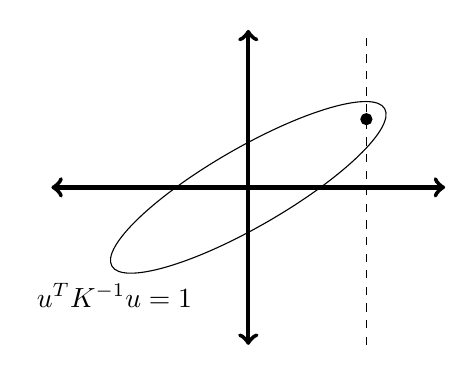
\begin{tikzpicture}
      \draw[rotate=30] (0,0) ellipse (2 and 0.5);
      \draw[ultra thick,<->] (-2.5,0) -- (2.5,0);
      \draw[ultra thick,<->] (0,-2) -- (0,2);
      \draw[dashed] (1.5,-2) -- (1.5,2);
      \node at (-1.7,-1.1) [below] {$u^T K^{-1} u = 1$};
      \draw[fill=black] (1.5,0.86603) circle (2pt);      
    \end{tikzpicture}
 \end{center}
 \caption{Prediction with uncertainty.}
 \label{fig1}
\end{figure}

\section{A framework for error analysis}

There is a simple trick that is useful for a wide variety of analyses
in approximation theory.  Let $\hat{f}$ be an approximate function
that we compute via some algorithm, and let $f$ be the true function
we are trying to approximate.  Then we will seek an intermediate
function $\tilde{f}$ --- not necessarily easy to compute, but
``nice'' somehow --- and we will write the error as
\[
  \hat{f}-f = (\hat{f}-\tilde{f}) + (\tilde{f}-f).
\]
Then we will try to reason about $\hat{f}-\tilde{f}$ and $\tilde{f}-f$
independently.  To make the idea a bit more concrete, let us now turn
to some examples.

\subsection{Bias-variance decomposition}

Suppose that for points $x_1, \ldots, x_m$ we have $y_i = f(x_i) + \epsilon_i$
for some random errors $\epsilon_i$ with mean zero and variance $\sigma^2$.
Based on the $y_i$, we compute an approximation $\hat{f}$ for $f$;
and because the $y_i$ involve some random noise noise the
approximation $\hat{f}$ will also be a random variable.  Let
$\tilde{f}(x) = \mathbb{E}_{\epsilon}[\hat{f}(x)]$ denote the mean
function, and write the error as $e = \hat{f}-f = u + v$ where
and $u = \hat{f}-\tilde{f}$ has zero mean and
$v = \tilde{f}-f$ has zero variance.  Hence,
\[
  \mathbb{E}[e^2]
  = \mathbb{E}[u^2 + 2uv + v^2] \\
  = \mathbb{E}[u^2] + 2\mathbb{E}[u] v + v^2 \\
  = \operatorname{Var}[u] + v^2,
\]
or, in terms of the original function,
\[
  \mathbb{E}[(\hat{f}-f)^2] = \operatorname{Var}[\hat{f}] + (f-\tilde{f})^2.
\]
This is usually called the {\em bias-variance decomposition} of the
squared error.  The first term on the right only has to do with
variance of the estimator due to measurement noise; the second term
has to do with the squared error of the average estimator.  Often,
there is a tradeoff between these two effects: when we move from
a simpler model to a more complex model (or decrease the
regularization of a complex model), we decrease the bias, but
increase the variance.  The variance term has to do
with how the algorithm amplifies noise, and we can typically estimate
it from a model for the noise terms $\epsilon$ {\em without} much
information about $f$.  In contrast, understanding the bias term
requires that we assume something more about $f$.

\subsection{Stability}

The bias-variance decomposition is useful for thinking about the
effects of random measurement noise on function approximation, but
what about systematic noise?  And what about that bias term?
We can treat these using the more general framework of
{\em stability} of the algorithm.

Denote {\em sampling} a function $f$ at points
$X = (x_1, x_2, \ldots, x_m)$ by
\[
  f_X = \begin{bmatrix} f(x_1) \\ f(x_2) \\ \ldots \\ f(x_m) \end{bmatrix},
\]
and let $\mathcal{A}$ denote the algorithm to approximate $f$ from
$f_X$.  We assume that $\mathcal{A}$ is {\em Lipschitz} with constant
$L$; that is, for any data vectors $u$ and $v$,
\[
  \|\mathcal{A}[v]-\mathcal{A}[w]\| \leq L\|v-w\|.
\]
In this context, we will also call $L$ the {\em stability constant}
for $\mathcal{A}$.  Note that stability is {\em independent} of the
data; it is purely a property of the algorithm.

Letting $u$ denote some uncertainty in the data (random or not), we have
\[
  \hat{f} = \mathcal{A}[f_X+u].
\]
Now let $\tilde{f}$ be some intermediate function, and write
\[
  \hat{f}-f =
    (\hat{f}-\mathcal{A}[\tilde{f}_X]) +
    (\mathcal{A}[\tilde{f}_X]-\tilde{f}) +
    (\tilde{f}-f).
\]
For any norm, the triangle inequality gives
\[
  \|\hat{f}-f\| \leq
    \|\hat{f}-\mathcal{A}[\tilde{f}_X]\| +
    \|\mathcal{A}[\tilde{f}_X]-\tilde{f}\| +
    \|\tilde{f}-f\|.
\]
Using the Lipschitz property of $\mathcal{A}$, we have
\[
  \|\hat{f}-f\| \leq
    L\|f_X+u-\tilde{f}_X\| +
    \|\tilde{f}-f\| +
    \|\mathcal{A}[\tilde{f}_X]-\tilde{f}\|.
\]
Specializing slightly to the max norm, we have
\[
  \|\hat{f}-f\|_\infty \leq
    (1+L)\|f-\tilde{f}\|_\infty + L\|u\|_\infty +
    \|\mathcal{A}[\tilde{f}_X]-\tilde{f}\|_\infty.
\]
Hence, the approximation algorithm is accurate if
\begin{itemize}
\item Some function $\tilde{f}$ is a good approximation to
  $f$ ($\|f-\tilde{f}\|_\infty$ small) and is itself accurately
  reconstructed from samples ($\|\mathcal{A}[\tilde{f}_X]-\tilde{f}\|$ small).
\item The stability constant $L$ is not too big.
\item The uncertainty $\|u\|_\infty$ is not too big.
\end{itemize}
This is an extremely powerful approach to error analysis, but
perhaps so general as to be confusing.  Let us make it concrete
by considering the case of interpolation or least-squares fitting
to a finite-dimensional function space.

\subsection{Quasi-optimality of interpolation and least squares}

% Bias-variance decomposition
% Consistency plus stability
% Analysis of interpolatory schemes

We now consider the algorithm
$\hat{f}(x) = \mathcal{A}[f_X + u]$ given by
\[
  \hat{f}(x) = \psi(x)^T c \mbox{ where }
  c = \operatorname{argmin} \sum_{i=1}^m (\psi(x_i)^T c - (f(x_i)+u_i))^2,
\]
where
\[
  \psi(x) =
  \begin{bmatrix} \psi_1(x) \\ \psi_2(x) \\ \vdots \\ \psi_N(x) \end{bmatrix} 
\]
is a column of basis functions for some $N$-dimensional approximation
space $\mathcal{F}$, and we assume that $m \geq N$.  In this case,
$\mathcal{A}$ is a linear map and $\mathcal{F}$ is the range space;
moreover, we have the exact reconstruction property
\[
  \forall g \in \mathcal{F}, \quad \mathcal{A}[g_X] = g.
\]
Now, define $\tilde{f}$ to be the {\em best possible approximation} to
$f$ in $\mathcal{F}$; that is $\|\tilde{f}-f\|$ is as small as
possible.  Using the exact reconstruction property together with
the decomposition in the last subsection, we have
\[
  \|f-\hat{f}\|_\infty \leq (1+L) \|f-\tilde{f}\|_\infty + L\|u\|_\infty.
\]
If $u$ is zero, this is a {\em quasi-optimality} result: we can get
within a factor of $(1+L)$ of the best possible error for any estimate
in the space!  Moreover, we can actually bound $L$ by the product of
$\max_x \sum_i |\psi(x)|$ --- which does not depend on the location of
the sample points --- and the matrix infinity norm for the
Moore-Penrose pseudoinverse in the least squares problem.

\section{Polynomial interpolation}

In order to test out our fancy error analysis frameworks, let us
consider the problem of {\em polynomial interpolation} on some
interval (for example, $[-1,1]$).  Let $\mathcal{P}_d$ denote the
$d+1$-dimensional space of polynomials of degree at most $d$.  For a
length $d+1$ list of interpolation points $X$, the polynomial
interpolation algorithm computes
\[
  \mathcal{A}[f] = p \in \mathcal{P}_d \mbox{ s.t.~}
  p_X = f_X.
\]
By our last result, we are within a factor of $1+L$ of the best
possible approximation, where $L$ is the Lipschitz constant for
the algorithm.

In the polynomial interpolation setting, the Lipschitz constant has a
special name: it is known as the {\em Lebesgue constant}, and it is
given by
\[
  L = \max_x \sum_{j=0}^d |l_j(x)|
\]
where the functions $l_j$ are the Lagrange polynomials, which are one
at the point $x_j$ and zero at the other points $x_i \neq x_j$; equivalently,
\[
  l_j = \mathcal{A}[e_j]
\]
where $e_j$ is the $j$th column of the identity matrix.  The Lebesgue
constant blows up exponentially with $d$ for equi-spaced points, but
only grows logarithmically with $d$ for the so-called {\em Chebyshev points}.

What about the best possible polynomial approximation?  According to
the Stone-Weierstrass theorem, the polynomials are dense in the
continuous functions on a closed interval, so best polynomial
approximations should converge to any continuous target function.  One
standard result that you may have seen in an earlier course on
scientific computing illustrates another trick we will see again soon:
write the error in function approximation as a difference between
two approximators.  For an arbitrary point $x'$, we write
\[
  f(x')-p(x') = q(x')-p(x')
\]
where $q \in \calP_{d+1}$ is the polynomial of degree $d+1$ that
interpolates $f$ at the points in $X$ {\em and} at $x'$.  We can write
this polynomial as
\[
  q(x) = p(x) + c \prod_{j=0}^d (x'-x_j),
\]
where the coefficient $c$ in front of the last term is determined by
the new interpolation condition:
\[
  f(x')-p(x') = q(x')-p(x') = c \prod_{j=0}^d (x'-x_j).
\]
The coefficient $c$ is sometimes written as $f[x_0, \ldots, x_d]$,
and it can be computed by Newton's {\em divided difference} formula;
an interesting feature is that if $f$ has $d+1$ continuous
derivatives, then
\[
  f[x_0, \ldots, x_d] = \frac{f^{(d+1)}(\xi)}{(d+1)!}
\]
at some intermediate $\xi$ between the largest and smallest of the
points in $\{x_i\}_{i=0}^d \cup \{x'\}$.  Thus, the error
in polynomial interpolation for very smooth functions can be written
in much the same way as the error in Taylor expansion for very smooth
functions, and a bound on the $d+1$ derivative implies an error bound.
In fact, it is sufficient to have that the $d$th derivative has a
Lipschitz constant $M$; in this case, assuming all the points $x_i$
lie in some interval $[a,b]$, we have the uniform approximation
bound over the interval
\[
  E_d[f; a, b] \equiv \max_{x \in [a,b]} |f(x)-p(x)|
  \leq \frac{M (b-a)^{d+1}}{(d+1)!}
\]
Unfortunately, this approach does not help us to reason about
interpolation of functions without so many derivatives, even though
we know by Stone-Weierstrass that they can be approximated by polynomials.

A collection of theorems collectively known as {\em Jackson
  inequalities} provides more detailed bounds on the error for the
best polynomial approximation: the error in approximating an $r$-times
differentiable function by a degree $d \geq r$ polynomial on an interval
$[a,b]$ satisfies the bound
\[
  E_d[f; a,b] \leq \frac{A_r(b-a)^r}{d^r}
    \omega\left( f^{(r)}; \frac{b-a}{d} \right)
\]
where $A_r$ is a constant depending only on $r$ and $\omega$ refers
to the {\em modulus of continuity} of the $r$th derivative.
For a general function $g$, the modulus of continuity is
\[
  \omega(g; h) = \sup_{x, |t| \leq h} |g(x+t)-g(x)|,
\]
and when $g$ is Lipschitz with constant $M$, we have
\[
  \omega(g; h) \leq Mh.
\]
Therefore if $f^{(r)}$ is Lipschitz with constant $M$, we have the
slightly simpler error bound
\[
  E_d[f; a,b] \leq \frac{A_r M (b-a)^{r+1}}{d^{r+1}}.
\]
When the function is complex analytic, another argument shows that we
have {\em exponential} convergence of the best polynomial
approximation\footnote{%
  {\em Exponential} convergence means that the error behaves like $O(\xi^d)$
  for some $\xi < 1$.  The best $\xi$ possible for optimal polynomial
  approximation to an analytic $f$ depends on the distance
  between the approximation interval $[a,b]$ and the closest
  singularity in the complex plane.  Convergence of the form $O(d^{-(r+1)})$ is
  {\em algebraic} convergence.
}.

Given that the stability constant (also called the Lebesgue constant)
for polynomial interpolation at equally spaced points {\em grows
  exponentially} with the number of points and our bounds on the best
approximation {\em do not decay exponentially} except for analytic
functions, we have not shown that polynomial interpolation will always
converge as we add more and more data points {\em even without
  uncertainty in the function values}.  In fact, it generally does not
converge\footnote{And it may not converge even for analytic functions
  if the domain of interest is too near a singularity in the complex
  plane.}.  Therefore, we usually avoid high-degree polynomial {\em
  interpolation} except at carefully chosen points (e.g.~the Chebyhsev
nodes), though we still use high-degree polynomials with {\em least
  squares} approximation.

\section{Piecewise polynomial approximation}

As we saw in the previous section, the error bounds for polynomial
approximation depend on the regularity, as measured by derivative
bounds; the degree $d$ of the polynomial; and the length $b-a$ of the
interval.  We can get better approximations by increasing the
polynomial degree, but this is a delicate business unless we can
decide the locations where we will have data.  An alternative is
to split the domain into smaller pieces, then approximate the function
by a different polynomial on each subdomain.
This is {\em piecewise polynomial approximation}.  We consider two
specific examples.

\subsection{DNNs and piecewise linear approximation}

The simplest possible approximation is a {\em piecewise linear}
interpolant.  In one dimension, for data given at adjacent points
$x \in [x_i, x_{i+1}]$, we use the approximation
\[
  \hat{f}(x) =
  \frac{x-x_i}{x_{i+1}-x_i} f(x_i) + \frac{x_{i+1}-x}{x_{i+1}-x_i} f(x_{i+1}).
\]
If the derivative is Lipschitz with constant $M$ on $[x_i, x_{i+1}]$,
then the error bound on that interval is
\[
  |\hat{f}(x)-f(x)| \leq \frac{Mh_i^2}{8},
\]
where $h_i = x_{i+1}-x_i$.  The error bounds in higher-dimensional
spaces are similar, if more complicated to derive: if
$\|H_f\|_2 \leq M$ then on a simplex with containment radius $r$
(the radius of the smallest ball containing the simplex), the error in linear
interpolation is at most $Mr^2/2$.

One way of writing linear interpolation (in 1D) for interpolation
points $x_1 \leq x_2 \leq \ldots \leq x_m$ is
\[
\hat{f}(x) =
f(x_1) + f[x_2,x_1] \psi(x-x_1) +
  \sum_{j=1}^n (f[x_j,x_{j+1}]-f[x_j,x_{j-1}]) \psi(x-x_{j+1})
\]
where $f[x,y] = (f(x)-f(y))/(x-y)$ and $\psi(x) = [x]_+$ is the
so-called {\em rectified linear unit} (ReLU) function.  That is, we
can build a fairly general class of piecewise linear approximations
by combining affine operations (simple shifts of $x$ in this case)
with an elementwise nonlinearity.  If we let $c$ denote the
coefficients in this expansion, $b$ be the vector of nodal
coordinates, and $e$ be the vector of all ones, we can write this
approximation compactly as
\[
  \hat{f}(x) = c^T \psi(ex-b) + f(x_1)
\]
where $\psi$ is applied elementwise.  This is a particularly simple
example of a {\em neural network}, an approximation scheme that
involves alternately applying affine maps ($x \mapsto ex-b$ and
$z \mapsto c^T z + f(x_1)$) and elementwise nonlinearities (in this
case through the map $\psi$).  More generally, we might write
\begin{align*}
  y^0 &= x \\
  y^{i+1} &= \psi(A^i y^i + b^i) \\
  \hat{f}(x) &= A^{l} y^l + b^l
\end{align*}
Each intermediate stage $y_{i+1}$ represents a vector of piecewise
linear functions of $x$ that are linearly mapped and then ``folded''
by the ReLU nonlinearity to produce a new piecewise linear function
with even more pieces.  Even modest size mappings can produce a
{\em lot} of linear pieces, though not a triangulation of the space.
Relatively shallow networks can reproduce general linear interpolation
schemes in more than one input variable, though with potentially wide
layers.  Of course, the name ``deep neural network'' is much more
impressive sounding than ``a type of piecewise linear approximation!''

\subsection{Cubic splines}

One step up from piecewise linear approximation is {\em piecewise cubic}
approximation: that is, we approximate $f$ by different cubic
functions on each interval $[x_i, x_{i+1}]$.  The space of cubic
functions is four-dimensional, so making the cubic agree with the
function values at the endpoints of the interval is not enough.
To make the approximation unique, one usually considers either
{\em Hermite} approximation, where $f(x_i)$ and $f'(x_i)$ are given
at each node; or a {\em cubic spline}, where we use only function values
but also make first and second derivatives match at
the nodal points.  This provides us with $4n-2$ conditions for $4n$
unknown.  Of several possible choices for the extra two
conditions, we will consider the ``natural'' conditions
$y''(x_1) = 0$ and $y''(x_n) = 0$.

As it turns out, the spline has a natural mechanical interpretation.
If we take a thin piece of wood along the $x$ axis and push it up and
down at points $x_i$ so that it is displaced by $f(x_i)$, the resting
shape that it takes on will be that of a spline.  We can see this as
solving the partial differential equation $u'''' = 0$ with appropriate
``free'' boundary conditions, or as minimizing the energy
\[
  \mathcal{E}[\hat{f}] = \frac{1}{2} \int_a^b |\hat{f}''(x)|^2 \, dx
\]
subject to the interpolation constraints.  This quadratic
form is not strictly positive definite -- there are two null
directions associated with arguments of the form $d_1 + d_2 x$,
which we can think of as ``rigid body modes''
(translation up and down for constant fields, rotation for linear).

There are several ways to write a spline.  With an eye to generalizing
to higher dimensions, we will use the version
\[
  \hat{f}(x) = d_1 + d_2 x + \sum_{i=1}^n c_i |x-x_i|^3.
\]
This function is clearly cubic between points, and also clearly has
two continuous derivatives everywhere.  The $n+2$ parameters are
determined by the function values and by the insistence that
$\psi''(x_1) = \psi''(x_n) = 0$; as it turns out, these conditions
can be rewritten as
\begin{align*}
  \sum_{i=1}^n c_i &= 0 &
  \sum_{i=1}^n c_i x_i &= 0.
\end{align*}
Putting the interpolation conditions together with these boundary
conditions, we have the linear system
\[
\begin{bmatrix}
  K_{XX} & P \\
  P^T & 0
\end{bmatrix}
\begin{bmatrix} c \\ d \end{bmatrix} =
\begin{bmatrix} f_X \\ 0 \end{bmatrix}
\]
where $f_X$ denotes the vector of function values (as before),
$P_{i1} = 1$ and $P_{i2} = x_i$, and $(K_{XX})_{ij} = |x_i-x_j|^3$.
The matrix $K_{XX}$ is a special case of a {\em kernel matrix},
which we will discuss in more detail next time.  In fact, the quadratic form
\[
  f_X^T K_{XX}^{-1} f_X
\]
is within a constant factor of the bending energy $\mathcal{E}[f]$,
so this set of equations is equivalent to the KKT equations for
minimizing the bending energy of $\hat{f}$ subject to the pointwise
constraints and to the constraint that $\hat{f}$ is ``discretely
orthogonal'' to the rigid body modes.

\end{document}
